\documentclass[compress]{beamer}
\usepackage{irbookslide}
\usepackage{irilmenau2}
\usepackage{tikz}
\usepackage{url}
\usepackage{ifxetex}
\RequireXeTeX
\usepackage{fontspec} % zahteva paket euenc
\usepackage{xunicode}
\usepackage{xltxtra}
\usepackage{polyglossia}
\usepackage{minted}
\usepackage{algorithmic}
%\setdefaultlanguage[script=Latin]{serbian}

\title{Analiza algoritama}
\author{Branko Milosavljević}
\institute{Katedra za informatiku, Fakultet tehničkih nauka, Univerzitet u
Novom Sadu}
\date{2014.}
\subject{Predavanja sa ASP}

\begin{document}

\frame{\titlepage}

\frame{
  \frametitle{Analiza algoritama}
  \begin{itemize}
    \item algoritam će od nekog ulaza proizvesti neki izlaz \\ \ \\ \ \\
    \item ULAZ $\rightarrow$ ALGORITAM $\rightarrow$ IZLAZ
  \end{itemize}
}
\frame{
  \frametitle{Vreme izvršavanja}
  \begin{itemize}
    \item većina algoritama transformiše objekte na ulazu u objekte na izlazu
    \item \myred{vreme izvršavanja} algoritma obično raste sa veličinom ulaza
    \item teško je izračunati prosečno vreme izvršavanja
    \item posmatraćemo najgori slučaj
    \begin{itemize}
      \item jednostavnije za analizu
      \item ključno za primene kao što su igre, finansije ili robotika
    \end{itemize}
  \end{itemize}
}
\frame{
  \frametitle{Vreme izvršavanja}
  \begin{center}
    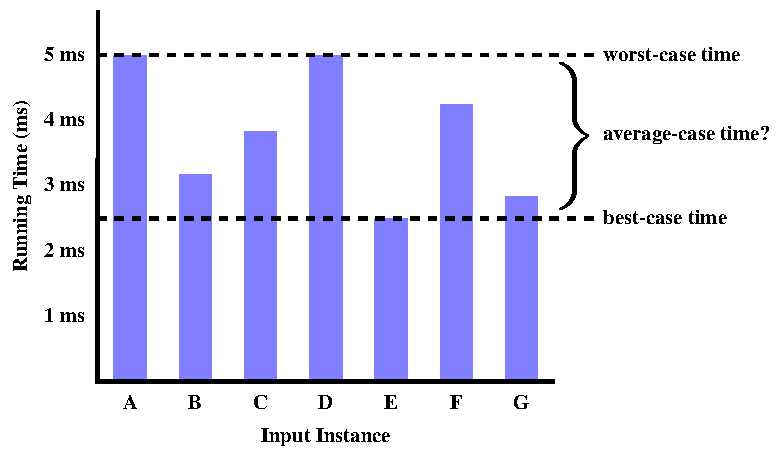
\includegraphics[width=10cm]{asp-01-pic01.pdf}
  \end{center}
}
\frame{
  \frametitle{Eksperimentalno proučavanje algoritama}
  \begin{itemize}
    \item napisati program koji implementira posmatrani algoritam
    \item pokrenuti program za različite veličine i strukturu ulaznih podataka
    \item meriti vreme izvršavanja
    \item analizirati rezultate
  \end{itemize}
}
\begin{frame}[fragile]
  \frametitle{Merenje vremena pomoću sistemskog sata}
\begin{minted}[linenos=false]{python}
from time import time
start_time() = time()
# ... run algorithm ...
end_time = time()
elapsed = end_time - start_time
\end{minted}  
\end{frame}
\frame{
  \frametitle{Analiza rezultata merenja}
  \begin{center}
    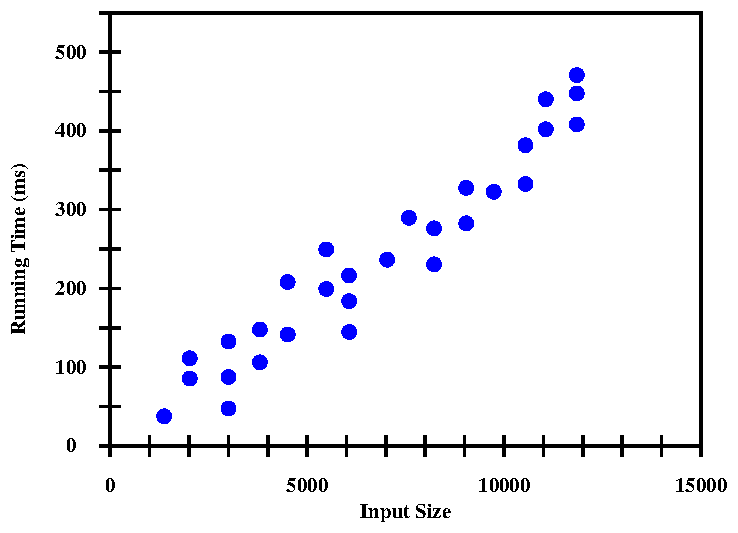
\includegraphics[width=10cm]{asp-01-pic02.pdf}
  \end{center}
}
\frame{
  \frametitle{Ograničenja eksperimentalnog pristupa}
  \begin{itemize}
    \item potrebno je implementirati algoritam --- može biti teško
    \item teško je predvideti rezultate za ulaze koji nisu obuhvaćeni
    eksperimentom
    \item za poređenje dva algoritma mora se koristiti identično hardversko
    i softversko okruženje
  \end{itemize}
}
\frame{
  \frametitle{Teorijski pristup}
  \begin{itemize}
    \item koristi se opis algoritma visokog nivoa umesto implementacije
    \item opisuje vreme izvršavanja kao funkciju veličine ulaza --- $n$
    \item uzima u obzir sve moguće ulaze
    \item omogućava procenu brzine algoritma nezavisno od korišćenog hardvera
    ili softvera
  \end{itemize}
}
\frame{
  \frametitle{Pseudokôd}
  \begin{itemize}
    \item opis algoritma visokog nivoa
    \item bolje strukturiran od prirodnog jezika
    \item manje detalja nego u stvarnom programu
    \item sakriva detalje vezane za dizajn programa
    \item poželjna notacija za opisivanje algoritama
  \end{itemize}
}
\begin{frame}[fragile]
  \frametitle{Pseudokôd}
  \begin{itemize}
    \item primer: pronalaženje najvećeg broja u nizu
  \end{itemize}
\begin{algorithmic}
\REQUIRE $A$: niz celih brojeva
\REQUIRE $n$: dužina niza
\STATE $currentMax \leftarrow A[0]$
\FOR{$i \leftarrow 1$ \TO $n-1$}
  \IF{$A[i] > currentMax$}
    \STATE $currentMax \leftarrow A[i]$
  \ENDIF
\ENDFOR
\RETURN $currentMax$
\end{algorithmic}
\end{frame}
\begin{frame}[fragile]
  \frametitle{Pseudokôd}
  \begin{itemize}
    \item kontrola toka
    \begin{itemize}
      \item \textbf{if} \ldots \textbf{then} \ldots [\textbf{else}] \textbf{end
      if} 
      \item \textbf{for} \ldots \textbf{do} \ldots \textbf{end for} 
      \item \textbf{while} \ldots \textbf{do} \ldots \textbf{end while} 
      \item \textbf{repeat} \ldots \textbf{until} \ldots 
    \end{itemize}
    \item izrazi 
    \begin{itemize}
      \item $\leftarrow$ dodela vrednosti 
      \item $=$ poređenje vrednosti 
      \item $n^2$ matematička notacija je OK 
    \end{itemize}
    \item vraćanje rezultata
    \begin{itemize}
      \item \textbf{return} vrednost 
    \end{itemize}
  \end{itemize}
\end{frame}
\frame{
  \frametitle{Sedam važnih funkcija $_1$}
  \begin{itemize}
    \item \myred{konstantna funkcija}
  \end{itemize}
  $$f(n) = c$$
  \begin{itemize}
    \item osnovna funkcija $g(n)=1$
    \item svaka druga može se prikazati kao $f(n)=c\cdot g(n)$
    \item može da opiše broj koraka potrebnih za neku od osnovnih operacija
    \item npr. sabiranje, dodela vrednosti, poređenje
  \end{itemize}
}
\frame{
  \frametitle{Sedam važnih funkcija $_2$}
  \begin{itemize}
    \item \myred{logaritamska funkcija}
  \end{itemize}
  $$f(n) = \log_b n$$
  \begin{itemize}
    \item za $b>1$
    \item za osnovu logaritma se najčešće koristi 2
    \item 2 se podrazumeva, tj. $\log n = \log_2 n$
    \item podela problema na dva dela: čest princip koji se koristi u
    algoritmima
  \end{itemize}
}
\frame{
  \frametitle{Sedam važnih funkcija $_3$}
  \begin{itemize}
    \item \myred{linearna funkcija}
  \end{itemize}
  $$f(n) = n$$
  \begin{itemize}
    \item kada treba obaviti prostu operaciju nad svakim od $n$ elemenata ulaza
    \item npr. poređenje broja sa svim elementima niza
  \end{itemize}
}
\frame{
  \frametitle{Sedam važnih funkcija $_4$}
  \begin{itemize}
    \item \myred{n-log-n funkcija}
  \end{itemize}
  $$f(n) = n \log n$$
  \begin{itemize}
    \item raste nešto brže od linearne funkcije
    \item i znatno sporije od kvadratne funkcije
    \item npr. najbrže sortiranje $n$ brojeva zahteva $n \log n$ vreme
  \end{itemize}
}
\frame{
  \frametitle{Sedam važnih funkcija $_5$}
  \begin{itemize}
    \item \myred{kvadratna funkcija}
  \end{itemize}
  $$f(n) = n^2$$
  \begin{itemize}
    \item npr. dve ugnježdene petlje 
    \item gde unutrašnja obavlja linearan broj operacija nad elementima ulaza
    \item a spoljna se izvršava linearan broj puta
    \item su proporcionalne sa $n^2$
  \end{itemize}
}
\frame{
  \frametitle{Sedam važnih funkcija $_6$}
  \begin{itemize}
    \item \myred{kubna funkcija}
  \end{itemize}
  $$f(n) = n^3$
  \begin{itemize}
    \item ređe se javlja od kvadratne, ali 
    \item predstavlja jednu klasu \myred{polinomijalnih} funkcija
  \end{itemize}
  $$f(n) = a_0 + a_1 n + a_2 n^2 + a_3 n^3 + \ldots + a_d n^d$$
}
\frame{
  \frametitle{Sedam važnih funkcija $_7$}
  \begin{itemize}
    \item \myred{eksponencijalna funkcija}
  \end{itemize}
  $$f(n) = b^n$$
  \begin{itemize}
    \item $b$ je baza
    \item $n$ je eksponent 
    \item često je $b = 2$
    \item najsporija
  \end{itemize}
}
\frame{
  \frametitle{Sedam važnih funkcija}
  \begin{center}
    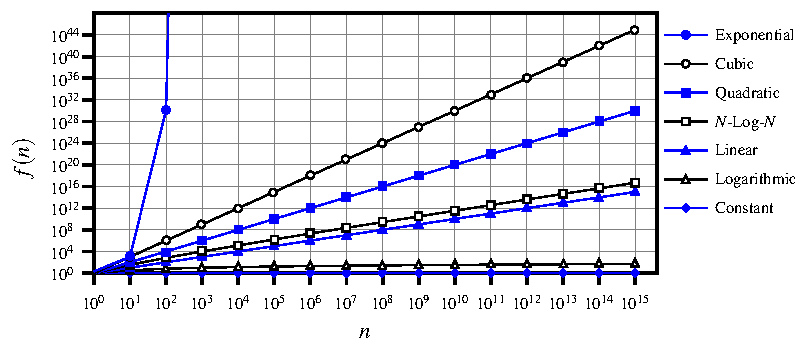
\includegraphics[width=11.5cm]{asp-01-pic03.pdf}
  \end{center}
}
\frame{
  \frametitle{Primitivne operacije}
  \begin{itemize}
    \item osnovne operacije koje izvršava algoritam
    \item prikazane u pseudokodu
    \item nezavisne od programskog jezika
    \item troše konstantnu količinu vremena
    \item na primer:
    \begin{itemize}
      \item izračunavanje izraza
      \item dodela vrednosti promenljivoj
      \item pristup elementu niza preko indeksa
      \item poziv funkcije
      \item vraćanje rezultata
    \end{itemize}
  \end{itemize}
}
\frame{
  \frametitle{Brojanje primitivnih operacija}
  \begin{itemize}
    \item analizom pseudokoda možemo odrediti maksimalan broj primitivnih
    operacija koje izvršava algoritam kao funkciju veličine ulaza
  \end{itemize}
}

\end{document}
